\documentclass[9pt]{beamer}
\mode<presentation>
{
	\usetheme{default}      
	\usecolortheme{default} 
	\usefonttheme{default}  
	\setbeamertemplate{navigation symbols}{}
	\setbeamertemplate{caption}[numbered]
} 

\usepackage[english]{babel}
\usepackage[utf8x]{inputenc}
\usepackage{graphicx}
%\usepackage[font=scriptsize,labelfont=scriptsize]{caption}
\usetheme{metropolis}

\title{fed2vec: a machine learning approach to forward guidance and market expectations}
\author{Temitope Akashoro\\
	Scott McNeil}
\date{\today}

\begin{document}
	
	\begin{frame}
		\titlepage
	\end{frame}
	
	
	\begin{frame}{Motivation: FOMC and Forward Guidance}
		
		\begin{columns}
			\begin{column}{0.5\textwidth}
				\begin{itemize}
					\item FOMC releases statements after meetings, detailing future policy
					\item Previous research (Campbell et al. 2012, Gurkaynak et al. 2005) study federal fund futures (FFF) as proxy
					\item Can we directly study these statements and their impact on market expectations?
				\end{itemize}
			\end{column}
			\begin{column}{0.5\textwidth}
				\begin{figure}
					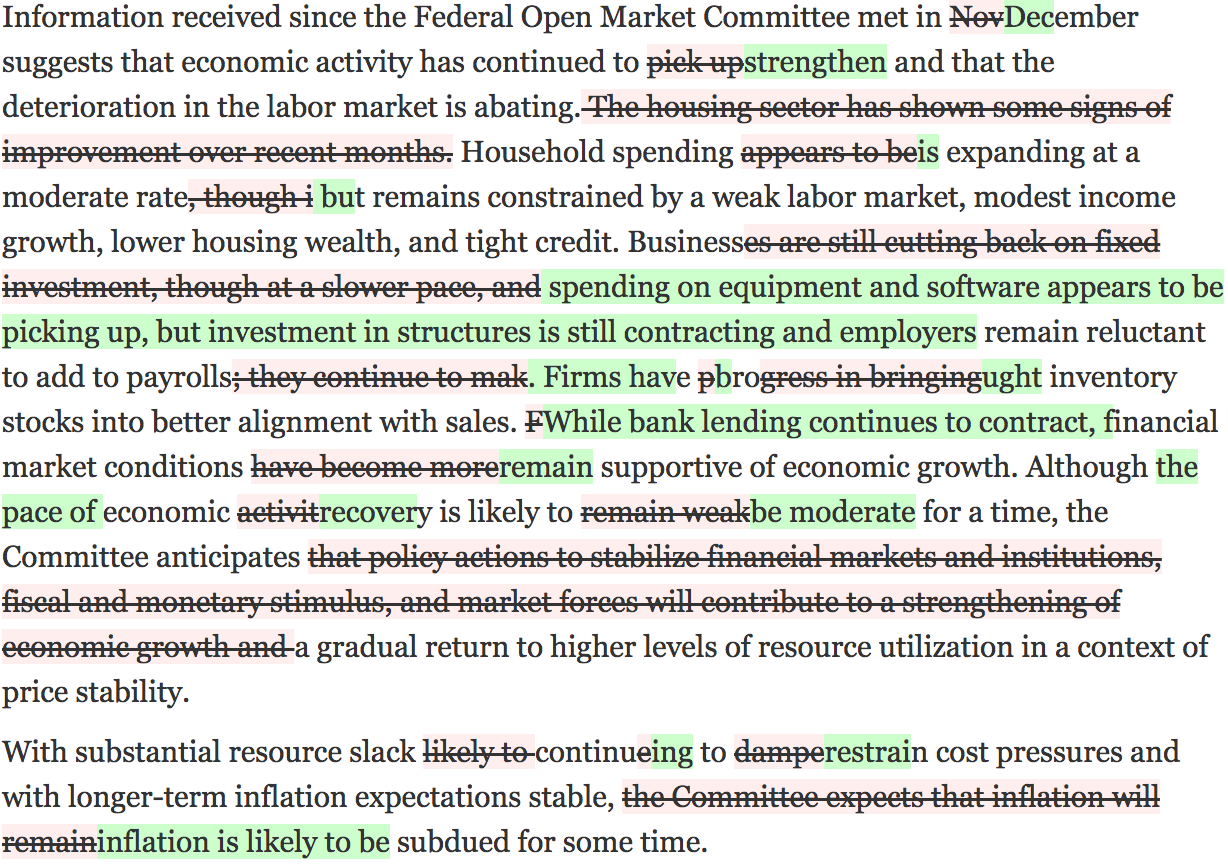
\includegraphics[width=1.05\textwidth]{fomcstatement.png}
					\caption{The \emph{Wall Street Journal's} \textquotedblleft Fed Statement Tracker\textquotedblright}
				\end{figure}
			\end{column}
		\end{columns}
		
	\end{frame}
	
	\begin{frame}{Methodology: word2vec and doc2vec}
		
		\begin{columns}
			\begin{column}{0.5\textwidth}
				\begin{itemize}
					\item Mikolov, et. al. (2013) and Le and Mikolov (2014) present word and document \textquotedblleft vectorization\textquotedblright
					\item Learn vector representation via word co-occurrence, dubbed ``word2vec"
					\item Similar words are clustered together while the distance between words also encode semantics
				\end{itemize}
			\end{column}
			\begin{column}{0.5\textwidth}
				\begin{figure}
					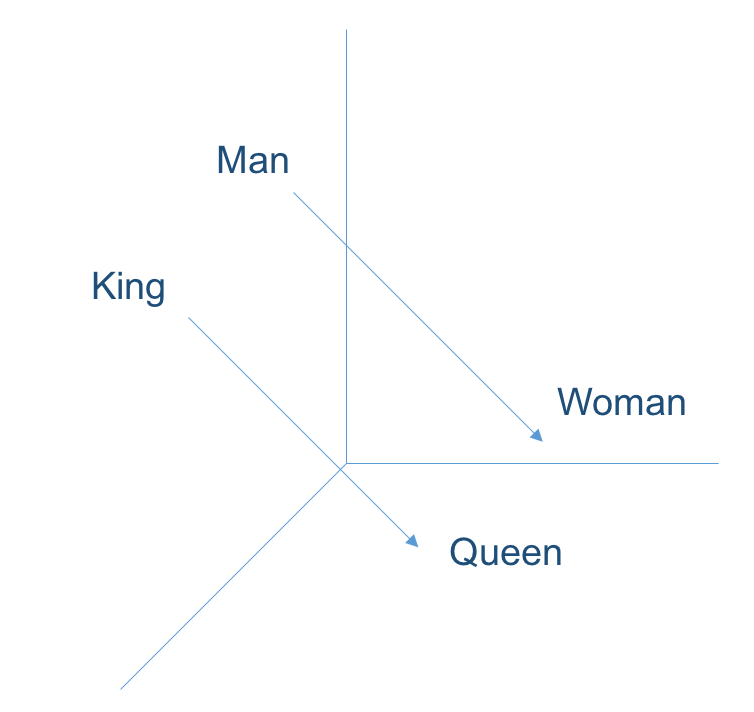
\includegraphics[width=\textwidth]{wordembedding.png}
					\caption{Result from Mikolov, et. al. (2013): king - him + her $\approx$ queen}
				\end{figure}
			\end{column}
		\end{columns}
		
		
	\end{frame}
	
	\begin{frame}{Data: Semantic Series}
		
		\begin{columns}
			\begin{column}{0.5\textwidth}
				\begin{itemize}
					\item Le and Mikolov (2014) extend this for documents, dubbed ``doc2vec''
					\item We use this on a large dataset of Federal Reserve documents to build document vectors
					\item Then we extract a time series of just FOMC statements and use PCA to reduce dimensionality
				\end{itemize}
			\end{column}
			\begin{column}{0.5\textwidth}
				\begin{figure}
					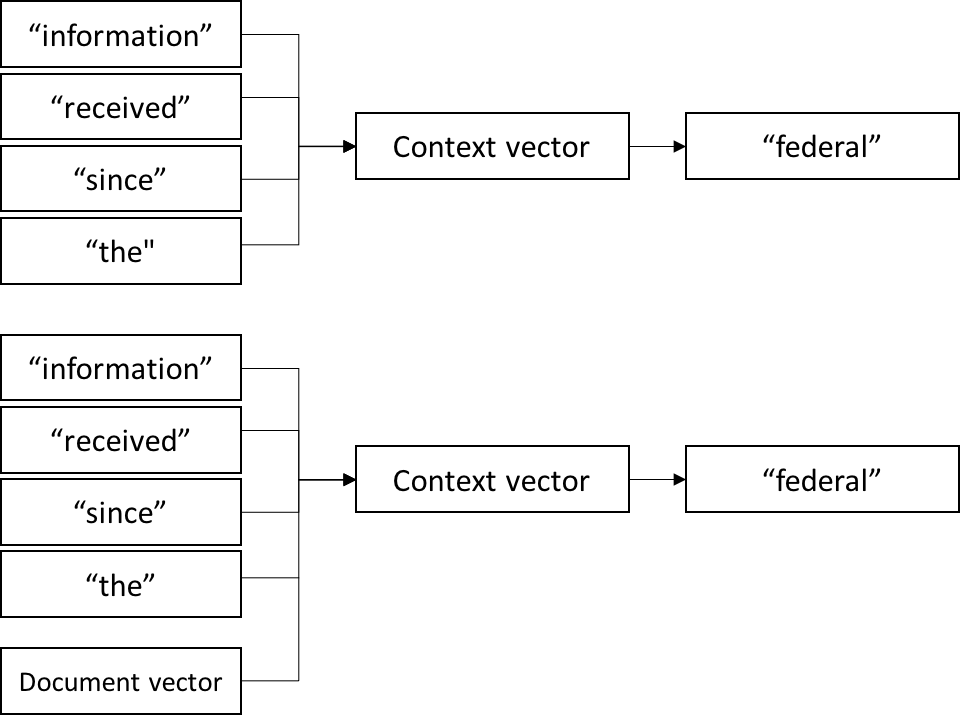
\includegraphics[width=0.8\textwidth]{doc2vec.png}
					\caption{Simplified version of word2vec (above) and doc2vec (below)}
				\end{figure}
			\end{column}
		\end{columns}
		
		
	\end{frame}
	\begin{frame}{Data: Federal Fund Futures and Federal Fund Rate}
	
		\begin{columns}
			\begin{column}{0.5\textwidth}
				\begin{itemize}
					\item Federal fund futures are a bet on the future value of the effective federal fund rate.
					\item Their value is equivalent to 100 minus the expected rate at a given month.
					\item For example $100-FFF6$ is the expected federal fund rate 6 months in the future.
				\end{itemize}
			\end{column}
			\begin{column}{0.5\textwidth}
				\begin{figure}
					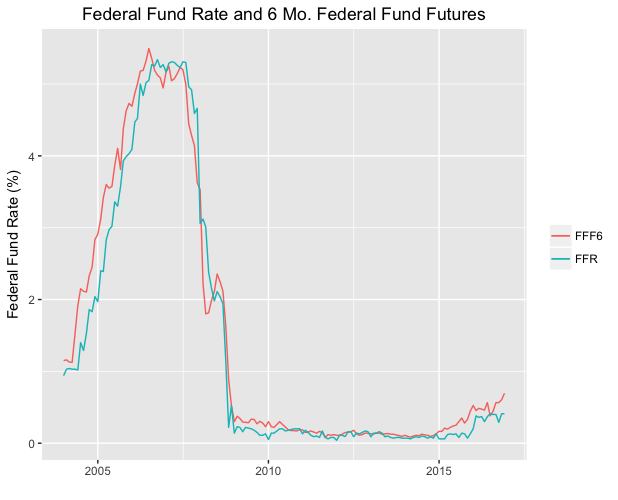
\includegraphics[width=0.8\textwidth]{ffrfff6.png}
					\caption{$FFF6$ and the federal fund rate from 2004 to 2016}
				\end{figure}
			\end{column}
		\end{columns}
	
	
	\end{frame}
	
	\begin{frame}{Data: Real Economy}
	
	\begin{columns}
		\begin{column}{0.5\textwidth}
			\begin{itemize}
				\item Also need to account for what agents know about the real economy
				\item Use Mccracken and Ng (2015), who provide updated set of 129 real economy time series
				\item Then use PCA to reduce this into just a few ``factors," based on FAVAR approach of Bernanke, et. al. (2005)
			\end{itemize}
		\end{column}
		\begin{column}{0.5\textwidth}
			\begin{figure}
				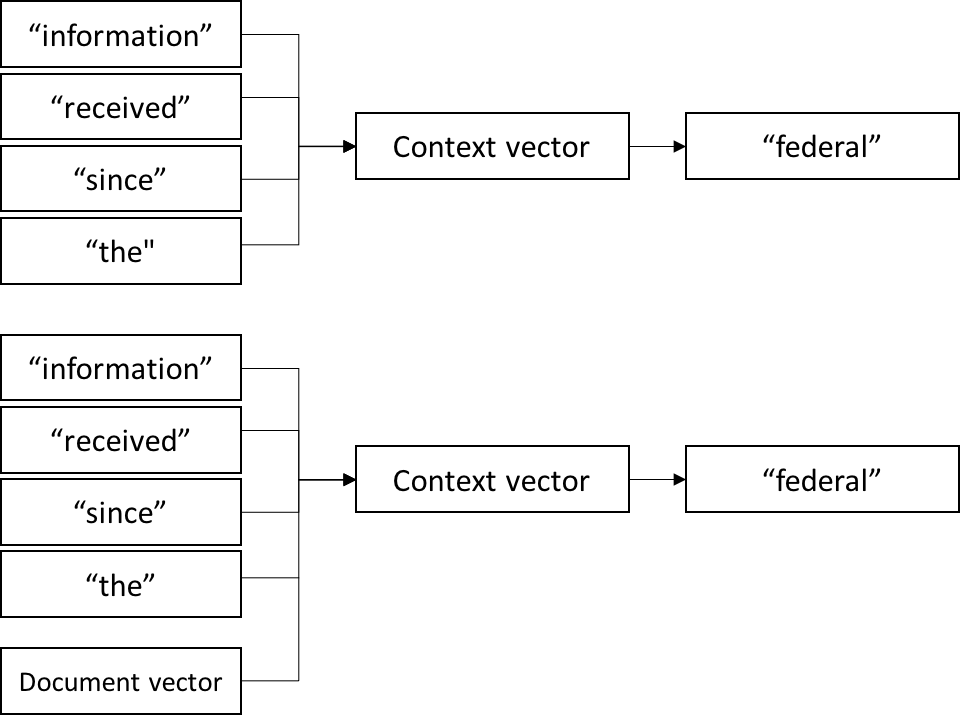
\includegraphics[width=0.8\textwidth]{doc2vec.png}
				\caption{Simplified version of word2vec (above) and doc2vec (below)}
			\end{figure}
		\end{column}
	\end{columns}
	
	
	\end{frame}

	
	\begin{frame}{Baseline Model}
		
		\begin{columns}
			\begin{column}{0.48\textwidth}
				\begin{itemize}
					\item We expect federal fund futures, FOMC statements and federal fund rate to be endogenous with contemporaneous effects \quad \quad \quad$\Rightarrow$ SVAR model
					\item $FFF$ and $R$ are unit root, so we use first difference
					\item Our full model is to the right, and we use a standard Cholesky and upper triangle method for identification
				\end{itemize}
			\end{column}
			\begin{column}{0.5\textwidth}
				\scriptsize\begin{align}
				&A_b\begin{bmatrix}
				\hat{S}_t\\
				\Delta R_t\\
				-\Delta FFF_t
				\end{bmatrix} =
				B_b\begin{bmatrix}
				\hat{S}_{t-1}\\
				\Delta{R}_{t-1}\\
				\Delta FFF_{t-1}
				\end{bmatrix} + \epsilon_{b,t} \nonumber \\
				&\hat{S}_t\text{: first principal component of semantic factors} \nonumber \\
				&\Delta R_t\text{: change in federal funds rate} \nonumber \\
				&\Delta FFF_t\text{: change in federal funds futures} \nonumber \\
				&\epsilon_{b,t}\text{: vec. of baseline, structural innovations} \nonumber \\
				&A_b\text{: $3\times 3$ square matrix of contemp. coeff.} \nonumber \\
				&B_b\text{: $3\times 3$ square matrix of lag coeff.} \nonumber
				\end{align}
			\end{column}
		\end{columns}
	\end{frame}

	\begin{frame}{Factor-Augmented Model}
	
	\begin{columns}
		\begin{column}{0.48\textwidth}
			\begin{itemize}
				\item We expect federal fund futures, FOMC statements and federal fund rate to be endogenous with contemporaneous effects \quad \quad \quad$\Rightarrow$ SVAR model
				\item $FFF$ and $R$ are unit root, so we use first difference
				\item Our full model is to the right, and we use a standard Cholesky and upper triangle method for identification
			\end{itemize}
		\end{column}
		\begin{column}{0.5\textwidth}
				\scriptsize\begin{align}
				&A_f\begin{bmatrix}
				\hat{S}_t\\
				\hat{F}_t\\
				\Delta R_t\\
				-\Delta FFF_t
				\end{bmatrix} =
				B_f\begin{bmatrix}
				\hat{S}_{t-1}\\
				\hat{F}_{t-1}\\
				\Delta R_{t-1}\\
				\Delta FFF_{t-1}
				\end{bmatrix} + \epsilon_{f,t} \nonumber \\
				&\hat{F}_t\text{: $m \times 1$ vector of factors} \nonumber \\
				&\epsilon_{f,t}\text{: vec. of augmented, structural innovations} \nonumber \\
				&A_f\text{: $m+3\times m+3$ square matrix of contemp. coeff.} \nonumber \\
				&B_f\text{: $m+3\times m+3$ square matrix of lag coeff.} \nonumber
				\end{align}
			\end{column}
		\end{columns}
	\end{frame}

	\begin{frame}{Baseline Results}
		\begin{columns}
			\begin{column}{0.48\textwidth}
				\begin{itemize}
					\item We're interested in the persistence of the impact of our semantic series on our federal fund futures series
					\item We find a persistent correlation between the first principal component of our semantic series and $FFF2$, $FFF4$ and $FFF6$
					\item We also reject a Granger causality test of the first principal component on all three
				\end{itemize}
			\end{column}
			\begin{column}{0.5\textwidth}
				\begin{figure}
					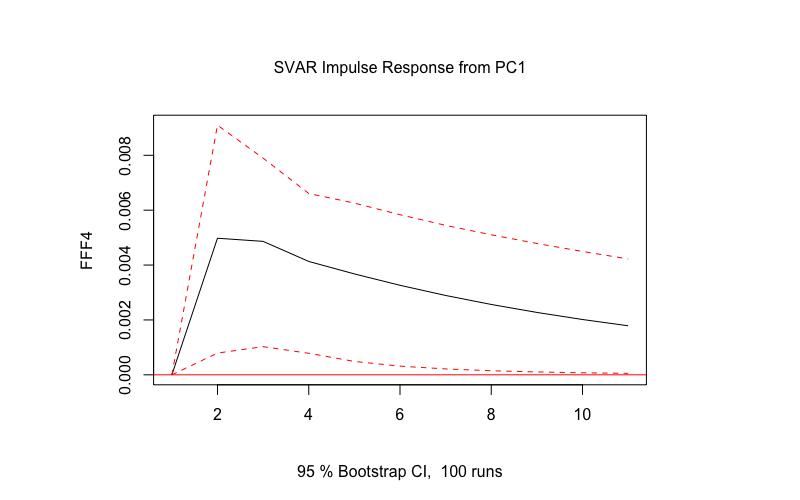
\includegraphics[width=0.8\textwidth]{baselineimpulse4.png}\\
					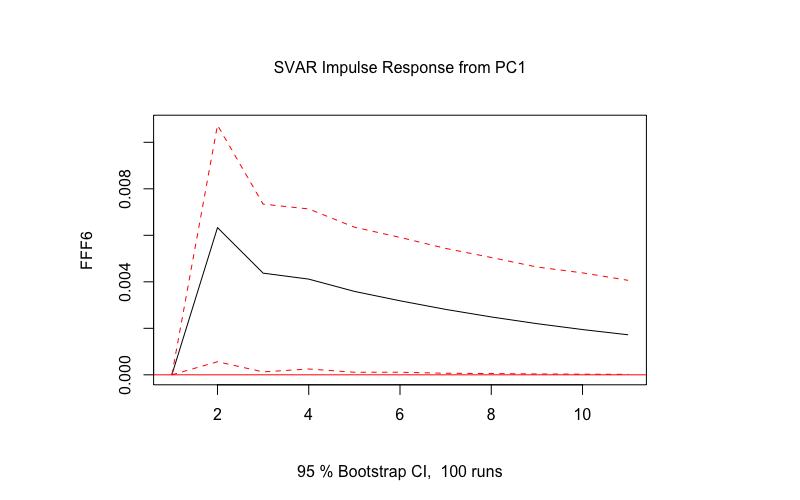
\includegraphics[width=0.8\textwidth]{baselineimpulse.png}
					\caption{Impulse response from first principal component of semantics on FFF4 and FFF6}
				\end{figure}
			\end{column}
		\end{columns}
	\end{frame}

	\begin{frame}{Factor-Augmented Results}
		\begin{columns}
			\begin{column}{0.48\textwidth}
				\begin{itemize}
					\item When we look at our factor augmented model, however, we no longer get significant results
					\item We also fail to reject a Granger causality test when we include our real economy factors
					\item This may be evidence that the FOMC is not actually adding information to the economy, but this is hard to interpret
				\end{itemize}
			\end{column}
			\begin{column}{0.5\textwidth}
				\begin{figure}
					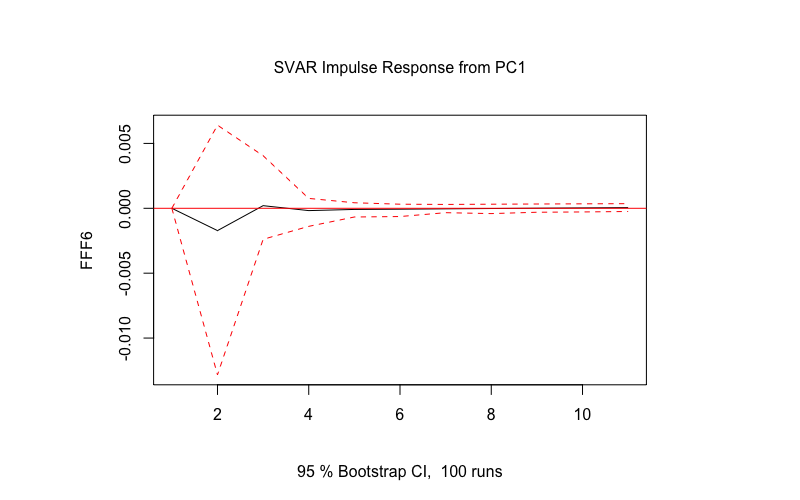
\includegraphics[width=\textwidth]{augmentedimpulse.png}
					\caption{Impulse response from first principal component of semantics on FFF6}
				\end{figure}
			\end{column}
		\end{columns}
	\end{frame}

	\begin{frame}{Conclusions and interpretation}
		\begin{columns}
			\begin{column}{0.48\textwidth}
				\begin{itemize}
					\item There appears to be some correlation between our semantics and the market expectations about future monetary policy
					\item Our semantics do correlate strongly with real economic variables, suggesting we're just measuring ``good economy, bad economy"
					\item We hoped that the word vectors would give us some direction, but don't give us anything clear at the moment
				\end{itemize}
			\end{column}
			\begin{column}{0.5\textwidth}
				\begin{figure}
					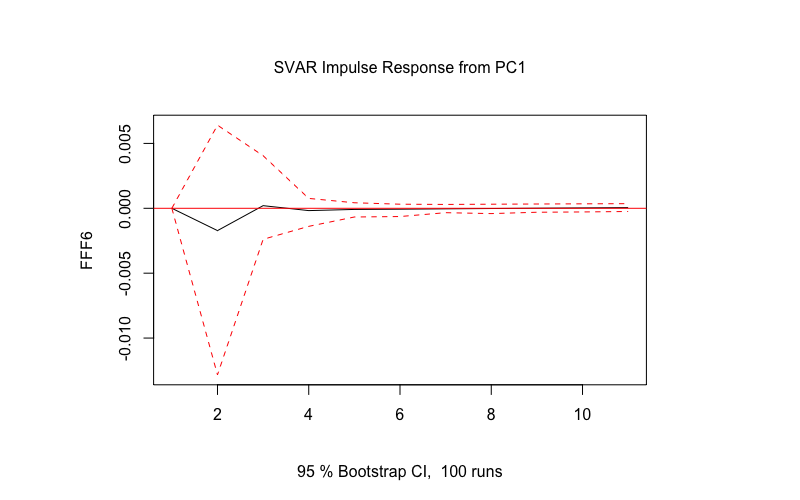
\includegraphics[width=\textwidth]{augmentedimpulse.png}
					\caption{Impulse response from first principal component of semantics on FFF6}
				\end{figure}
			\end{column}
		\end{columns}
	\end{frame}

	\begin{frame}{Issues and next steps}
		\begin{columns}
			\begin{column}{0.48\textwidth}
				\begin{itemize}
					\item One issue is our dimensionality reduction: the principle components of our semantic series don't explain a lot of variation

					\item It's possible we simply don't have a large enough corpus for the doc2vec algorithm to work properly
					\item One possible approach is to use the event study approach of Gurkaynak et al. (2005) to find dimensions that correspond to ``surprise factor"
				\end{itemize}
			\end{column}
			\begin{column}{0.5\textwidth}
				\begin{figure}
					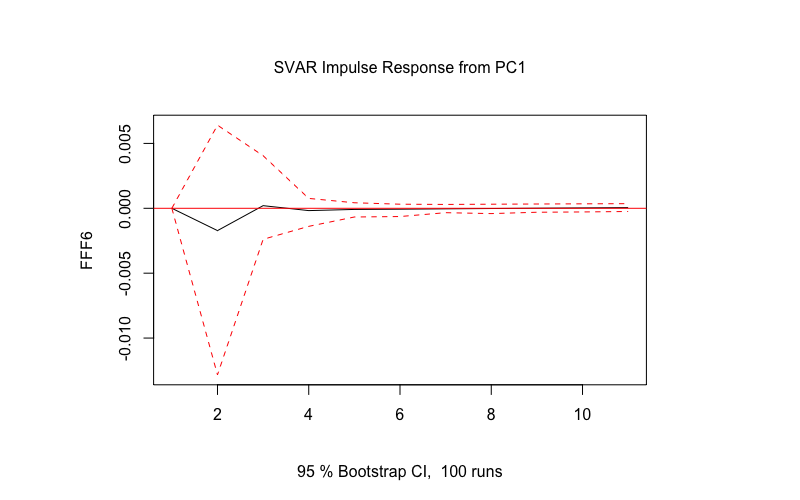
\includegraphics[width=\textwidth]{augmentedimpulse.png}
					\caption{Impulse response from first principal component of semantics on FFF6}
				\end{figure}
			\end{column}
		\end{columns}
	\end{frame}
	
	\begin{frame}{References}
		
\nocite{gurkaynak2005actions}
\nocite{campbell2012macroeconomic}
\nocite{le2014distributed}
\nocite{mikolov2013efficient}
\nocite{bernanke2005measuring}

\setbeamertemplate{bibliography item}[text]
\setbeamerfont{bibliography item}{size=\scriptsize}
\setbeamerfont{bibliography entry author}{size=\scriptsize}
\setbeamerfont{bibliography entry title}{size=\scriptsize}
\setbeamerfont{bibliography entry location}{size=\scriptsize}
\setbeamerfont{bibliography entry note}{size=\scriptsize}
\bibliographystyle{plain}
\bibliography{references}
		
	\end{frame}
	
\end{document}
